\documentclass[tikz,border=2mm]{standalone}
\usetikzlibrary{matrix}

\begin{document}

% One kind of arrow
%
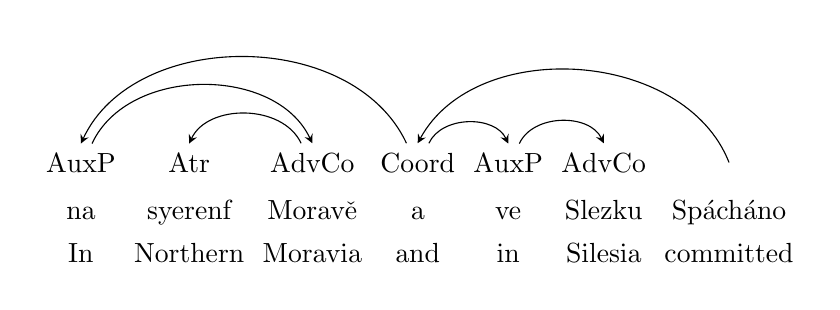
\begin{tikzpicture}[-stealth]

\matrix (word) [matrix of nodes,
			nodes in empty cells,
			execute at empty cell=\node{\strut};]
{
AuxP	& Atr			& AdvCo		& Coord	&AuxP	& AdvCo	&			\\
na	& syerenf		& Morav\v e 	& a 		& ve 		& Slezku	& Sp\'ach\'ano	\\
In 	& Northern	& Moravia		& and	& in 		& Silesia	& committed	\\
};

\draw (word-1-1.60)	 to [bend left=65] (word-1-3.north);
\draw (word-1-3.120)	to 	[bend right=65]	(word-1-2.north);
\draw (word-1-4.120)	to 	[bend right=65]	(word-1-1.north);
\draw (word-1-7.90)		to 	[bend right=65]	(word-1-4.north);
\draw (word-1-4.60) 		to 	[bend left=65] 		(word-1-5.north);
\draw (word-1-5.60) 		to 	[bend left=65]	 	(word-1-6.north);

\end{tikzpicture}

% Another kind of arrow
%

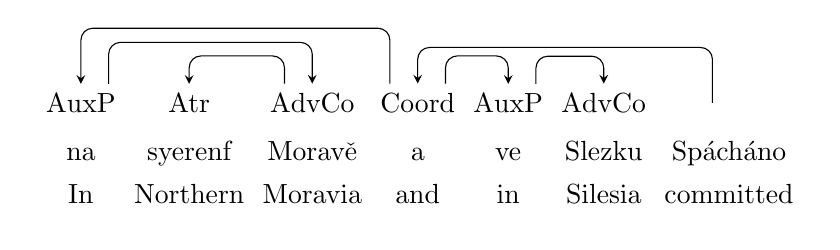
\begin{tikzpicture}[-stealth,rounded corners=1ex]
\tikzstyle{nudge right}=[xshift=6pt]
\tikzstyle{nudge left}=[xshift=-6pt]

\matrix (word) [matrix of nodes,
			nodes in empty cells,
			execute at empty cell=\node{\strut};]
{
AuxP	& Atr			& AdvCo		& Coord	&AuxP	& AdvCo	&			\\
na	& syerenf		& Morav\v e 	& a 		& ve 		& Slezku	& Sp\'ach\'ano	\\
In 	& Northern	& Moravia		& and	& in 		& Silesia	& committed	\\
};

\draw ([nudge right] word-1-1.60)	-- ++(0pt,15pt) -| 	(word-1-3.north);
\draw ([nudge left] word-1-3.120)	-- ++(0pt,10pt) -|	(word-1-2.north);
\draw ([nudge left] word-1-4.120)	-- ++(0pt,20pt) -|	(word-1-1.north);
\draw ([nudge left] word-1-7.90)	-- ++(0pt,20pt) -|	(word-1-4.north);
\draw ([nudge right] word-1-4.60) 	-- ++(0pt,10pt) -| 	(word-1-5.north);
\draw ([nudge right] word-1-5.60) 	-- ++(0pt,10pt) -|	 (word-1-6.north);

\end{tikzpicture}

\end{document}